\begin{task}{3, Bifurcations in higher dimensions}

The solution and plots for this task can be found in \verb|task3/non_linear_2_d.ipynb| for the first equation and in \verb|task3/non_linear_2_params.ipynb| for the second equation. Finally, some specific plotting utilities are implemented in \verb|task3/zero_convergence_plotter.py| by means of the ZeroConvergencePlotter class.

This task mostly concerns visualizing things. The task was accomplished using two python notebooks. For the visualization of the orbits it was decided to use the \verb|scipy.integrate.solve_ivp| solver.

\begin{figure}[H]
    \centering
    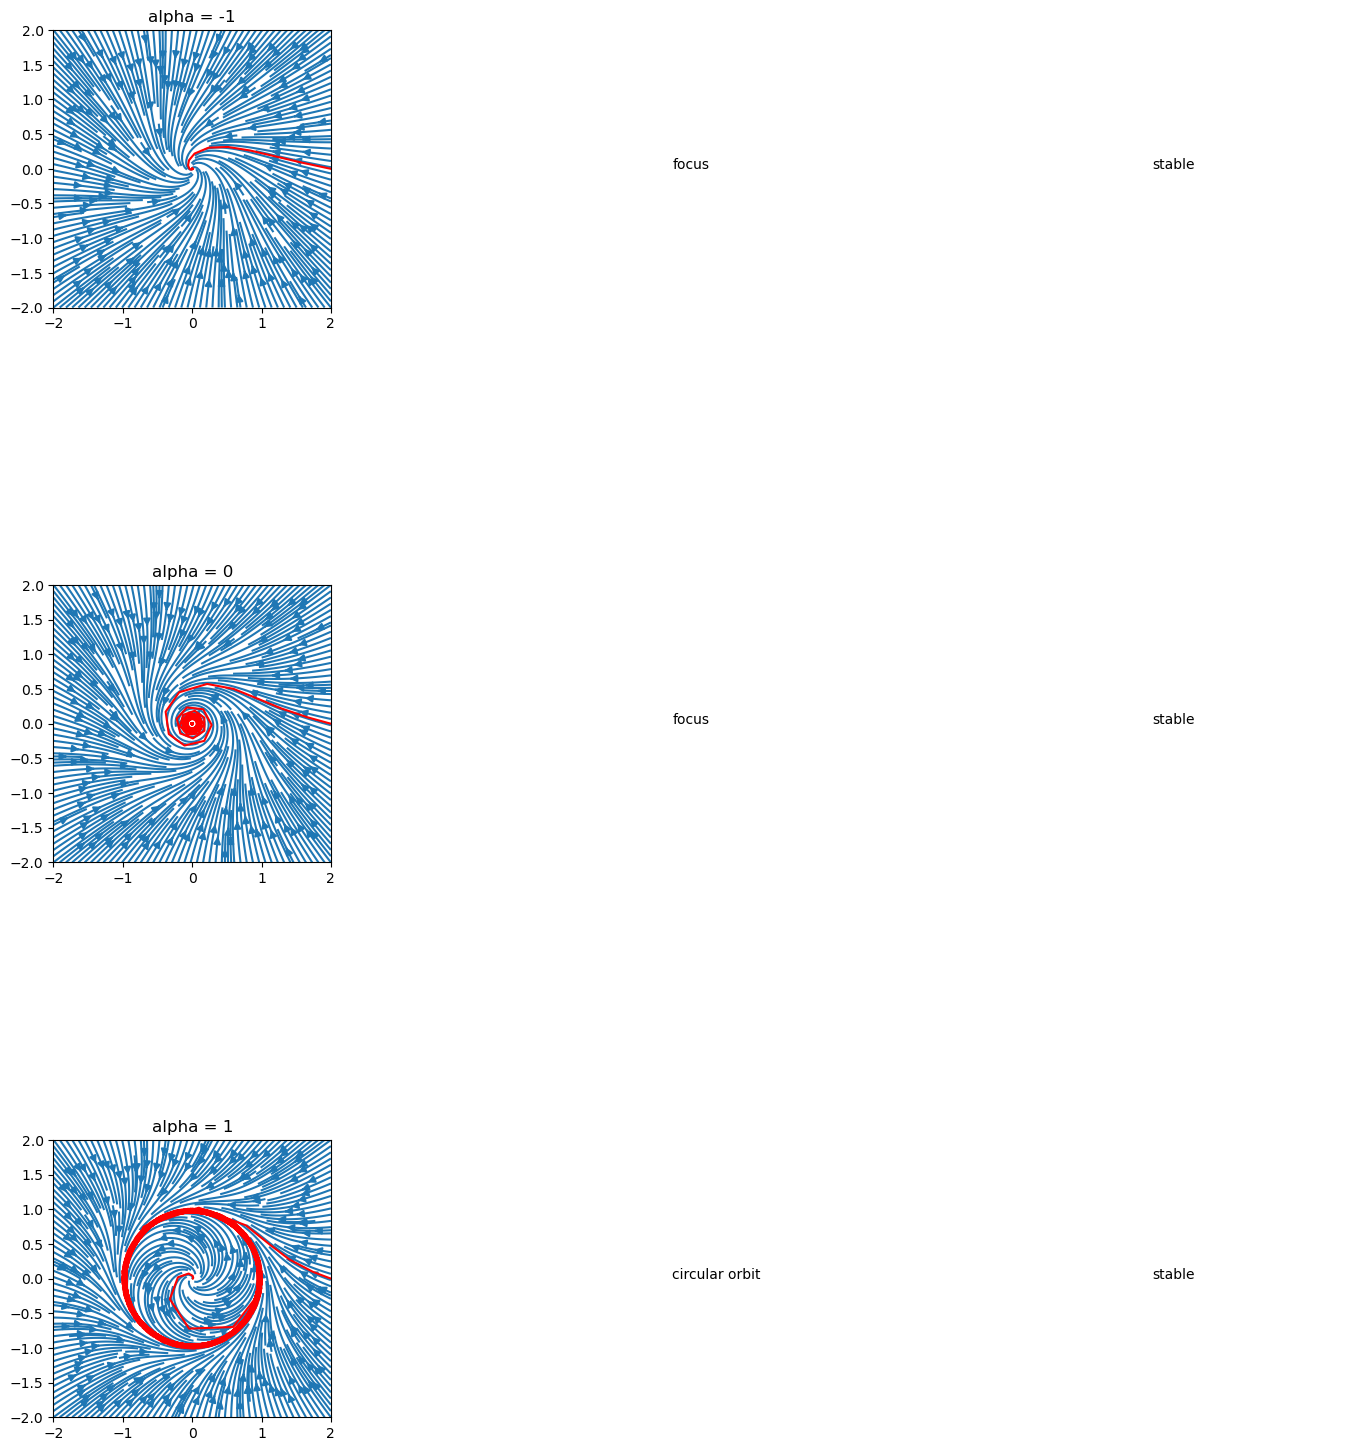
\includegraphics[width=0.8\textwidth]{images/bfdhopf.png}
    \caption{Phase diagrams of the system at different values.}
    \label{fig:bfdhopf}
\end{figure}

We can see in Figure \ref{fig:bfdhopf} that the systems at $\alpha = -1$ and $\alpha = 0$ simply have one stable focus at $(0,0)$. The system at $\alpha = 1$ has a stable orbit at $x^2+y^2 = 1$.

\begin{figure}[H]
    \centering
    \subfigure[the orbit that trajectory starting at $(2,0)$ settles into]{
    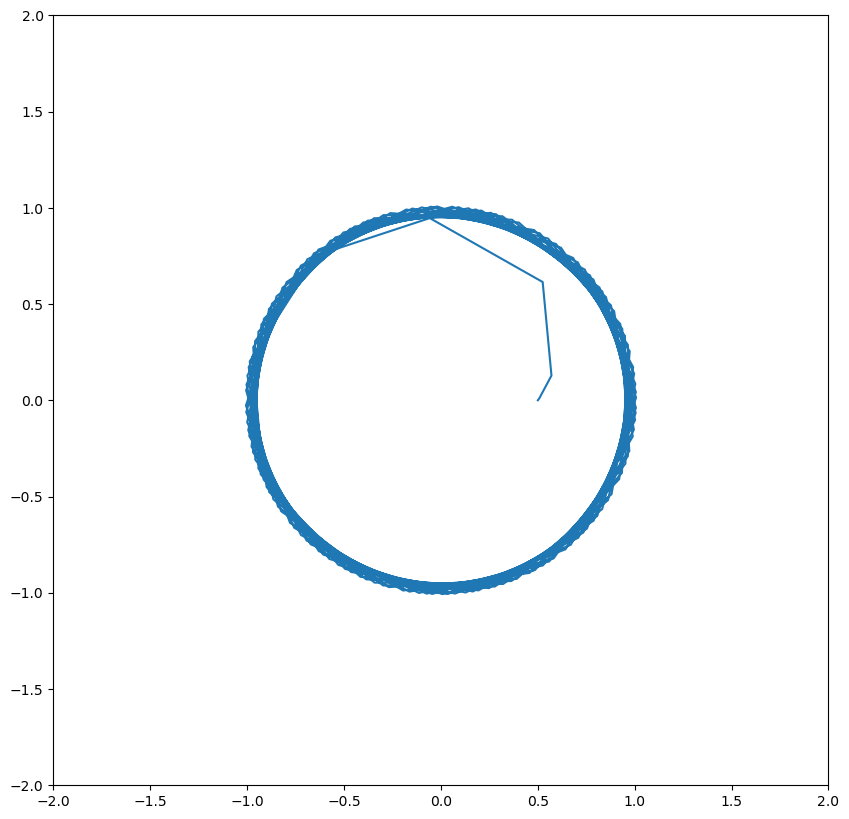
\includegraphics[width=0.4\textwidth]{images/orbit2000.png}}
    \subfigure[the orbit that trajectory starting at $(0.5,0)$ settles into]{
    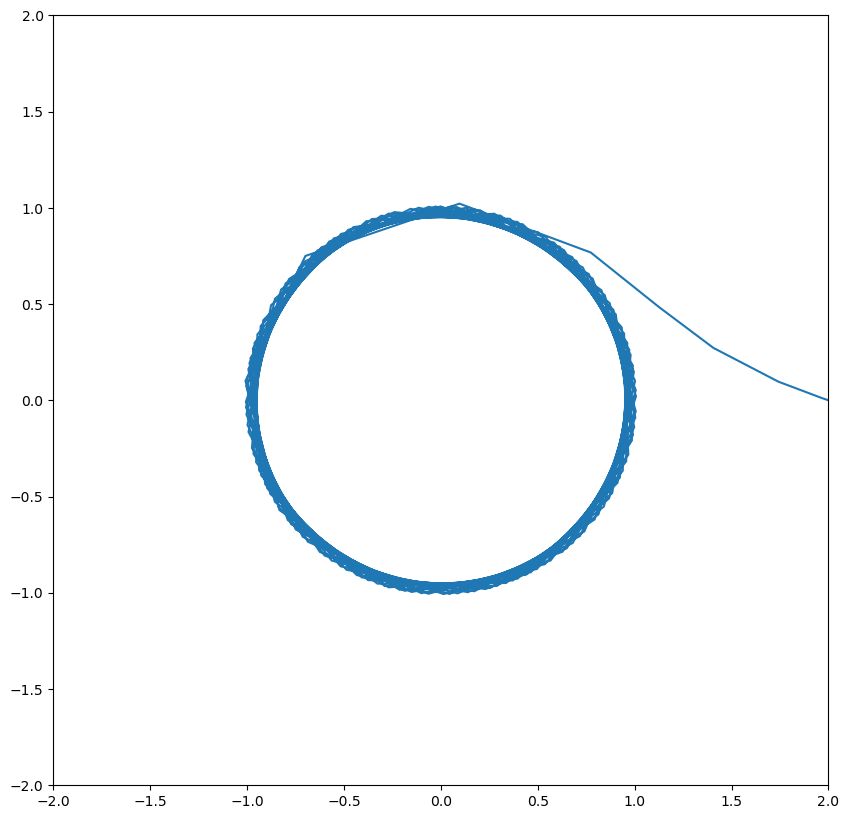
\includegraphics[width=0.4\textwidth]{images/orbit0500.png}}
    \caption{Orbits of the system for $\alpha = 1$.}
    \label{fig:orbits}
\end{figure}

We can see in Figure \ref{fig:orbits} that trajectories starting at both these points settle in the stable orbit at $x^2+y^2 = 1$.

We can construct Figure \ref{fig:f} through the procedure outlined in the assignment. That is we sample $(x, \alpha_2)$ uniformly and then plot the surface as a function $\alpha_1$ = $-((\alpha_2)x - x^3)$. We also plot a different plot where we sample $(x, \alpha_2)$ and then take $\alpha_1$ in steps of given size.

\begin{figure}[H]
    \centering
    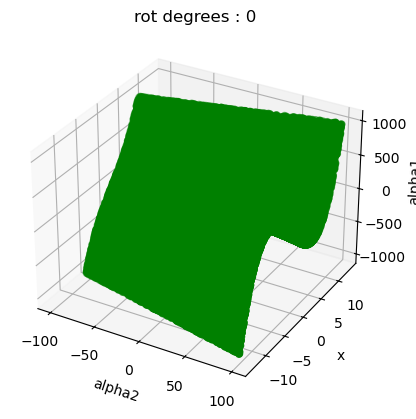
\includegraphics[width=0.4\textwidth]{images/fork0.png}
    \caption{3D plot of the bifurcation surface}
    \label{fig:f}
\end{figure}

The cusp cannot be seen in the diagram \ref{fig:f}. It is called cusp bifurcation because in the parameter space we can separate the area where there are 3 equilibria from the area where there is only 1 equilibrium using two curves, these meet at the cusp point.
\end{task}